\documentclass[mathpazo]{cicp}

\usepackage{graphicx}
\usepackage{amsmath}
\usepackage{amssymb}
\usepackage{amsthm}
\usepackage[dvips]{epsfig}
\usepackage{color}
\usepackage{multirow}
\DeclareGraphicsExtensions{.pdf,.png,.jpg,.eps}

%
% Cross-referencing
%
% Theorem--like environments
\newtheoremstyle{theoremlike}{3pt}{3pt}{\itshape}{}{\bfseries}{.}{.5em}{}
\theoremstyle{theoremlike}
\theoremstyle{definition}
\theoremstyle{remark}

\newtheorem{corollary}[theorem]{Corollary}
\newtheorem{lma}{Lemma}
\newtheorem{thm}{Theorem}
\newtheorem{cor}{Corollary}
\newtheorem{prop}{Proposition}
\newtheorem{hyp}{Hypothesis}
\newtheorem{cond}{Condition}

\newcommand{\Eq}[1]{Eq.~\eqref{#1}}
\newcommand{\Eqs}[1]{Eqs.~\eqref{#1}}
\newcommand{\Fig}[1]{Fig~\ref{#1}}
\newcommand{\Table}[1]{Table~\ref{#1}}
\newcommand{\Sec}[1]{Sec.~\ref{#1}}
\newcommand{\Subsec}[1]{Subsection~\ref{#1}}
\newcommand{\Secs}[1]{Secs.~\ref{#1}}

%
% Latin abbreviations
%

\newcommand{\cf}{{\it cf.}\ }
\newcommand{\eg}{{\it e.g.},\ }
\newcommand{\etal}{{\it et~al}.\ }
\newcommand{\etc}{{\it etc}}
\newcommand{\ie}{{\it i.e.},\ }
\newcommand{\via}{{\it via}\ }
\newcommand{\vs}{{\it vs.}\ }
\newcommand{\FronTier}{\textit{Fron\hspace{-2pt}T\hspace{-1pt}ier\hspace{2pt}}}

%
% Notation
%

\newcommand{\half}{\mathchoice
 {\tfrac{1}{2}} \frac{1}{2} {\frac{1}{2}} {1/2}}
\newcommand{\quarter}{\mathchoice
 {\tfrac{1}{4}} \frac{1}{4} {\frac{1}{4}} {1/4}}
\newcommand{\bfrac}[2]{\displaystyle
        \frac{\displaystyle #1}{\displaystyle #2}}
\newcommand{\pderiv}[2]{\mathchoice
 {\frac{\partial #1}{\partial #2}} {\partial #1/\partial #2}
 {\frac{\partial #1}{\partial #2}} {\partial #1/\partial #2} }
\newcommand{\oderiv}[2]{\mathchoice
 {\frac{d #1}{d #2}} {d #1/d #2} {\frac{d #1}{d #2}} {d #1/d #2} }

\newcommand{\tderiv}[3]{\pderiv{#1}{#2}\Bigm|_{#3}}

\newcommand{\vfrac}{\beta}
\newcommand{\energy}{e}
\newcommand{\intenergy}{\epsilon}
\newcommand{\vel}{\mathbf{v}}
\newcommand{\zhat}{\widehat{z}}
\newcommand{\vhat}{\widehat{v}}
\newcommand{\kp}{{k^\prime}}
\newcommand{\muv}{\mu^v}
\newcommand{\mup}{\mu^p}
\newcommand{\mupv}{\mu^{pv}}
\newcommand{\Log}{\ln}
\newcommand{\vavg}[1]{\overline{#1}}
\newcommand{\mavg}[1]{\widetilde{#1}}
\newcommand{\vect}[1]{\mathbf{#1}}

%%%%%%%%%%%%%%%%%%%%%%%%%%%%%%%
%%%%%% Document Start %%%%%%%%%
%%%%%%%%%%%%%%%%%%%%%%%%%%%%%%%

\begin{document}

\title{Application of GPU to Three Computational Models}

\author[Qiangqiang Shi \etal]{
Qiangqiang Shi\affil{1}\comma\corrauth,
Yiyang Yang\affil{1},
Xiaolin Li\affil{1}
}

\address{\affilnum{1}\ Department of Applied Mathematics and Statistics,
Stony Brook University, Stony Brook, NY 11794--3600, United States of America.}
\emails{{\tt qqshi@ams.sunysb.edu} (Qiangqiang Shi),
{\tt yiyang@ams.sunysb.edu} (Yiyang Yang),
{\tt linli@ams.sunysb.edu} (Xiaolin Li)}

\begin{abstract}
In this paper, we introduced the application of Graphics Processing
Unit (GPU)-based algorithms for high performance computation of mathematical
models in FronTier++. In the first case, the one-dimensional gas dynamics
problem is solved by Weighed Essentially Non-Oscillatory (WENO) scheme,
we achieved 7-20x speedup for different mesh sizes on 1 GPU. In the
second case, the spring model for fabric dynamics is studied, the
GPU code is about 10-20 times faster than the non-GPU code for different
mesh sizes. In the last case, a GPU enhanced numerical algorithm for
American option pricing under generalized hyperbolic distribution
was studied. Using one GPU, we have achieved 2x speedup for the price
of single option and 100x speedup for multiple options.
\end{abstract}

\keywords{GPGPU, gas dynamics, spring model, American option pricing }

\maketitle

%%%%%%%%%%%%%%%%%%%%%%%%%%%%%%%%%
%%%%%%  SECT Introduction  %%%%%%
%%%%%%%%%%%%%%%%%%%%%%%%%%%%%%%%%

\section{Introduction}

\subsection{Introduction to GPU computing}
Graphics Processing Units (GPU) computing \cite{kirk2010programming} is
the use of a GPUs together
with CPUs to accelerate general-purpose scientific and engineering
applications. Joint CPU/GPU application is a powerful combination
because CPUs consist of a few cores optimized for serial processing,
while GPUs consist of thoudands of smaller, more efficient cores designed
for parallel performance. GPU computing offers unprecedented application
performance by offloading compute-intensive portions of the application
to the GPU, while the remainder of the code still runs on CPU. 
\Fig{fig:GPU-acceleration-code-str} demonstrates the structure of hybird
GPU/CPU code. From the viewpoint of a user, applications simply run
remarkably faster.

\begin{figure}[htb]
\centering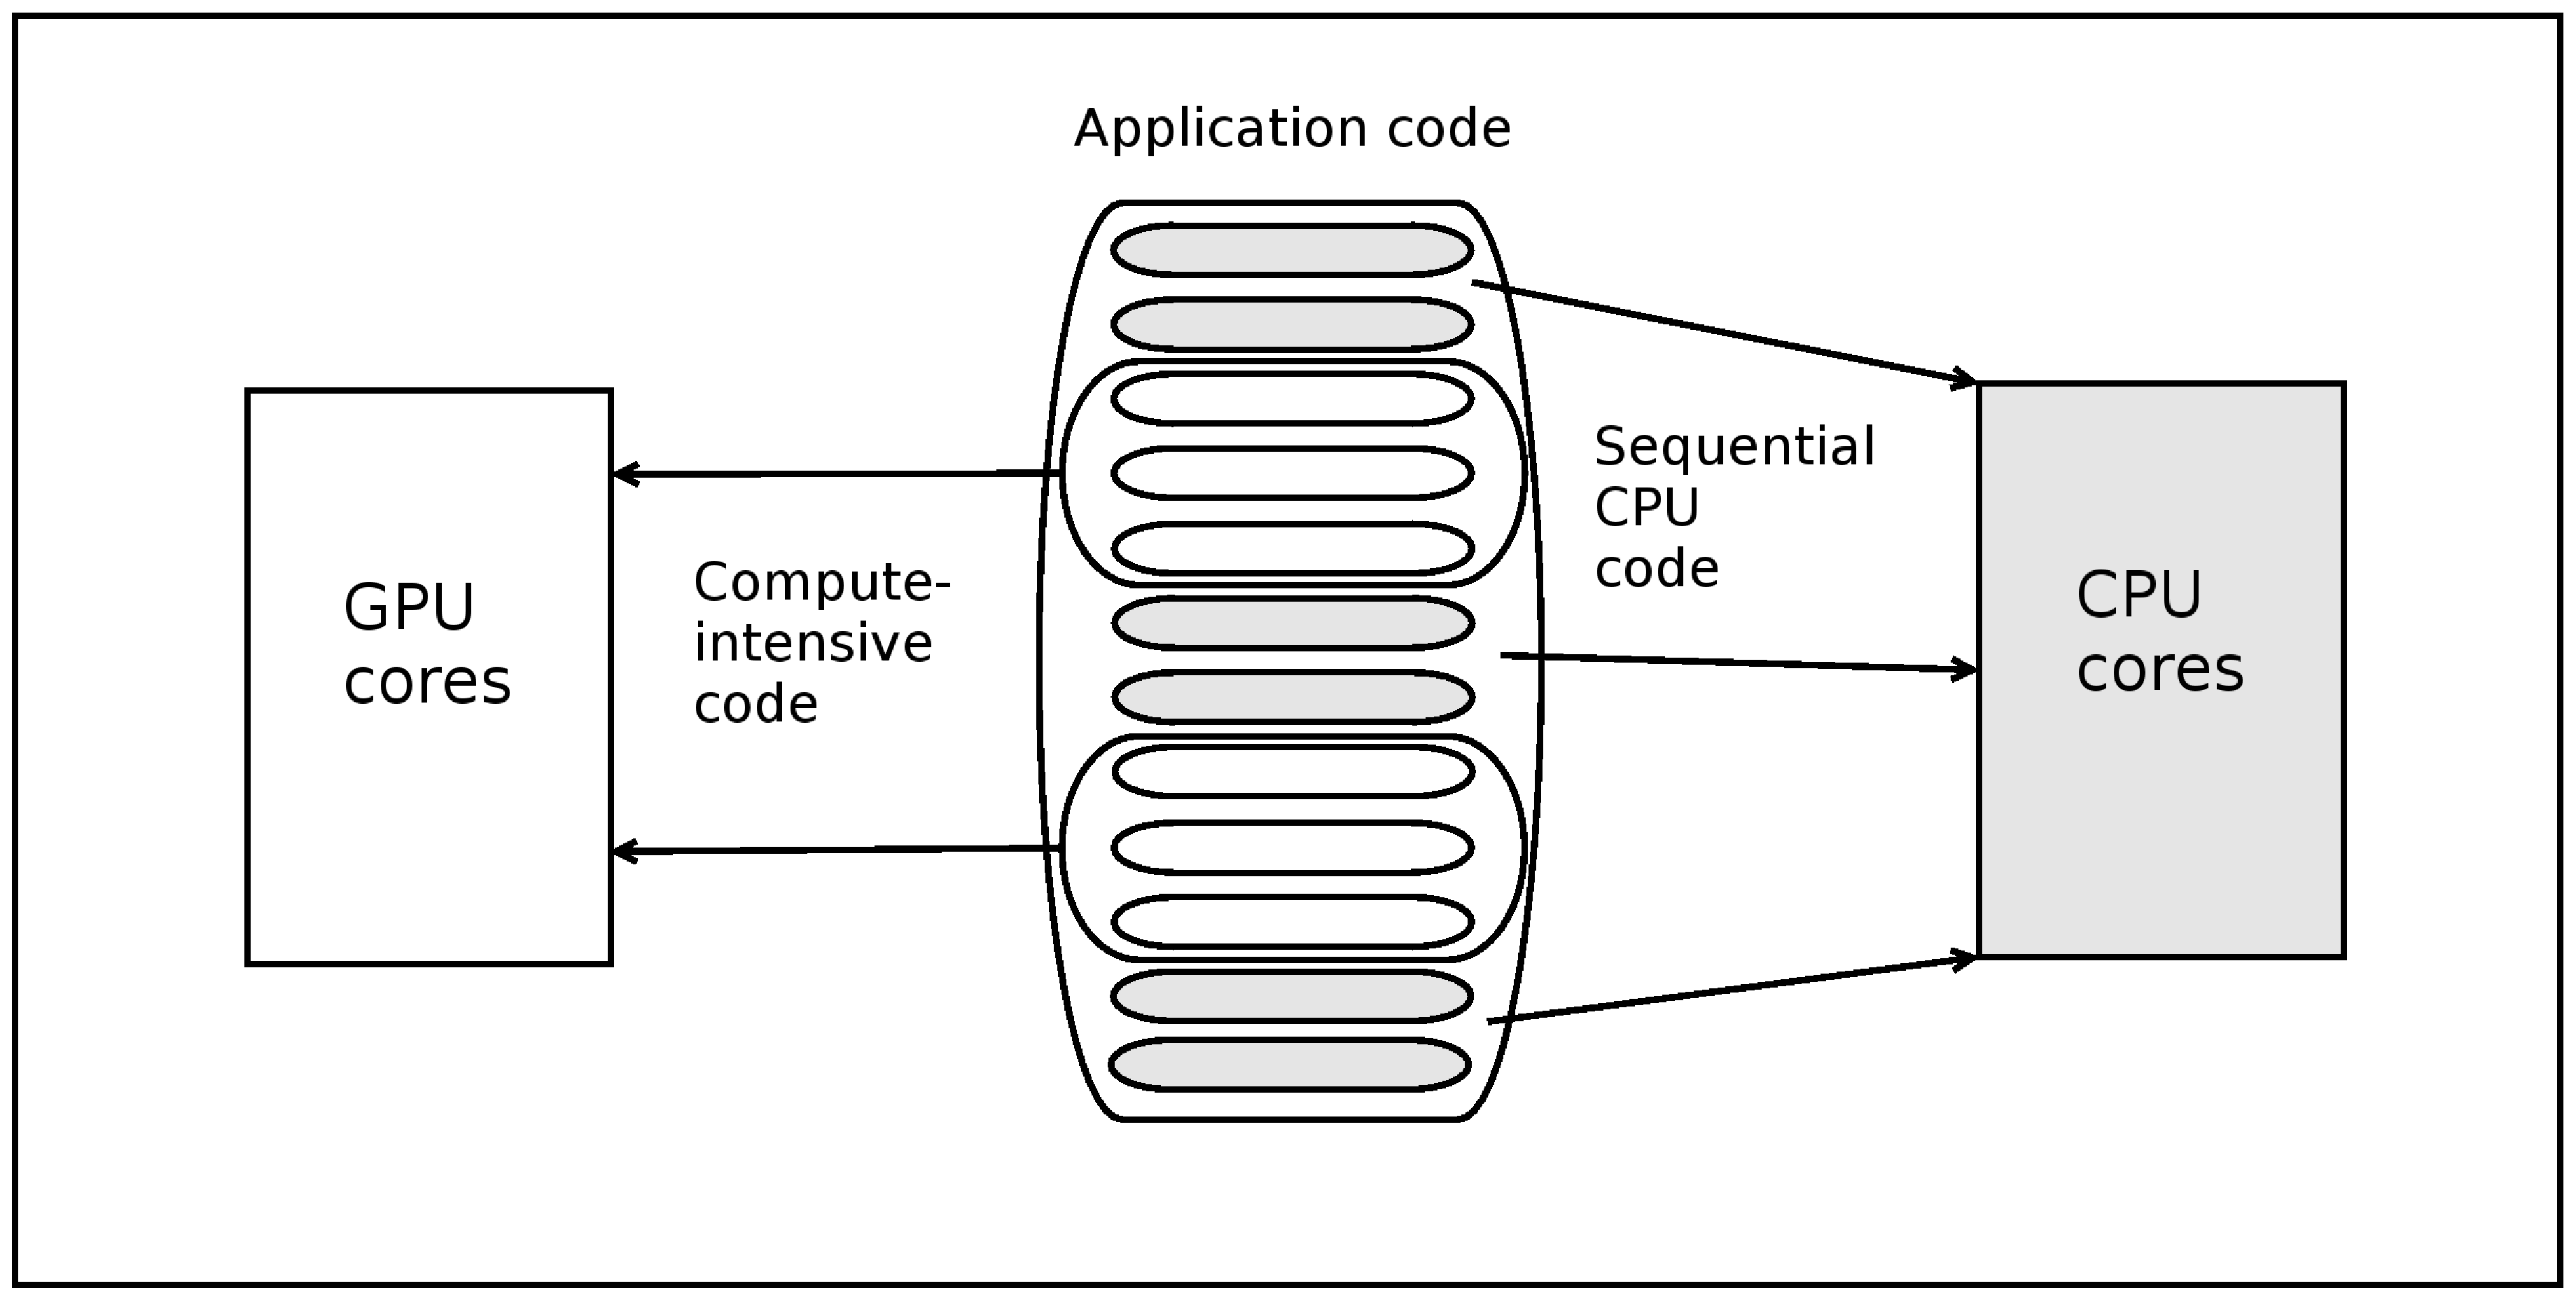
\includegraphics[scale=0.2]{fig_gpu_acceleration}
\caption{
\label{fig:GPU-acceleration-code-str}
GPU acceleration code stucture }
\end{figure}

\subsection{Related research}
GPU computing has become a more and more popular research topic in 
the past few years and voluminous studies have found that the 
speedups GPUs delivered are substantial compared to CPUs. 

\subsection{Experiment platform}
Both the CPU and the GPU studies were implemented on a dell 
precision T7600 Workstation with dual Intel Xeon 
E5-2687W CPUs and dual NVIDIA Quadro 6000 graphics cards. 
The Intel Xeon E5-2687W CPU is the latest multi-threaded multi-core 
Intel-Architecture processor. It offers eight cores on the same die running 
at 3.10 GHz. The Intel Xeon E5-2687W processor cores feature an
out-of-order super-scalar microarchitecture, with newly added 2-way 
hyper-threading. In addition to scalar units, it also has 4-wide SIMD units
that support a wide range of SIMD instuctions. Each has a separate 32KB L1 
cache for both instructions and data and a 256 KB unified L2 data cache.
All eight cores share an 20 MB L3 data cache. The Intel Xeon E5-2687W 
processor also features an on-die memory controller that connects to four 
channels of DDR memory.
Each Quadro 6000 graphics card consists of 14 streaming multiprocessors (SMs)
running at 1.15 GHz that share a single 768 KB L2 cache and 6 GB global
memory on the device. Each SM consists of 32 streaming processors (SPs),
a 48 KB shared memory and 32768 32-bit registers. Fedrora 18 with kernel 
3.9.2-200, CUDA Toolkit 5.0 and GCC 4.7.2 were used in the computations.
Table \ref{tab:Test-Environment} shows the hardware structure of our
computer. \Fig{fig:system-arch} illustrates the architecture of the 
computational platform and \Fig{fig:gpu-arch} demonstrates the 
architecture of multi-GPU devices.

\begin{table}[htb]
\centering
\caption{
A Dell Precision T7600 Workstation with dual NVIDIA Quadro 6000 graphics 
cards was used to set up the test environmet.
\label{tab:Test-Environment}
}
\begin{tabular}{|c|c|p{9cm}|}
\hline \hline
\multirow{6}{*}{{\small Hardware}} & \multirow{3}{*}{{\small CPU}}
& {\small Dual Eight Core XEON E5-2687W, 3.1GHz}\\
&  & {\small 64GB DDR3}\\
&  & {\small 32KB x 16 L1 Cache, 256KB x 16 L2 Cache, 20MB x 2 L3 Cache}\\
\cline{2-3}
& \multirow{3}{*}{{\small GPU}}
& {\small Dual Quadro 6000 with 14 multiprocessor, 448 cores, 1.15Hz}\\
&  & {\small 6GB global memory, 64 KB constant memory}\\
&  & {\small 48KB shared memory and 32768 registers per multiprocessor}\\
\hline
\multirow{3}{*}{{\small Software}} & {\small OS}
& {\small Fedora 18 with kernel 3.9.2-200.fc18.x86\_64}\\
 & {\small Compiler} & {\small gcc version 4.7.2 }\\
 & {\small CUDA} & {\small CUDA Toolkit 5.0}\\
\hline \hline
\end{tabular}
\end{table}

\begin{figure}[htb]
\centering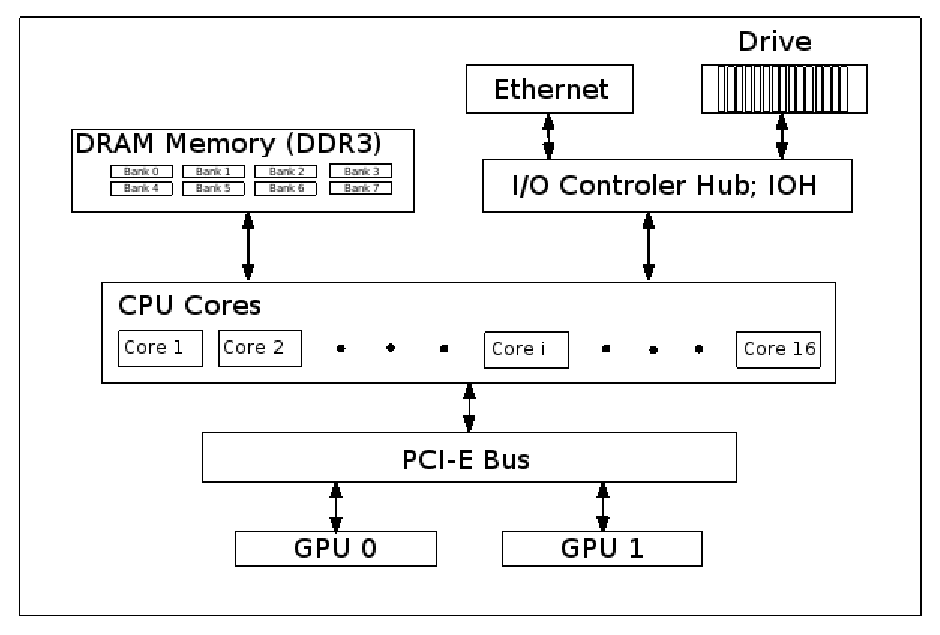
\includegraphics[scale=0.71]{fig_system_arch}
\caption{
\label{fig:system-arch}
Architecture of the experiment platform. The Host part has 16 
hyper-threading supported CPU cores and 64GB DRAM. The Device 
part consists of double NVIDIA Quadro 6000 graphics cards.
The host part and the device part were connected by the PCIe Bus.}
\end{figure}

\begin{figure}[htb]
\centering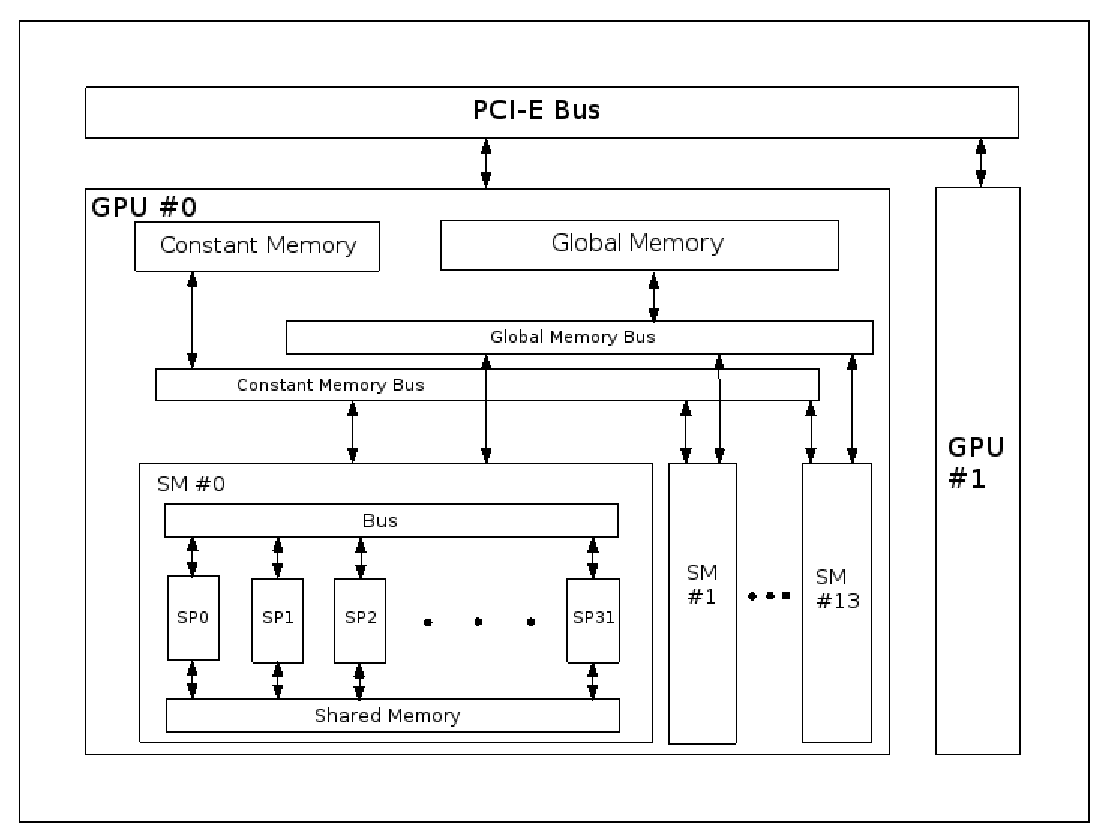
\includegraphics[scale=0.60]{fig_gpu_arch}
\caption{
\label{fig:gpu-arch}
Architecture of multi-GPU device. Each GPU hardware consists of 
memory (global, constant, shared) and 14 SMs.
Each SM consists of 32 SPs and can run 1536 threads simultaneously.}
\end{figure}

\section{GPU application to gas dynamics}

\section{GPU application to spring model}

\section{GPU application to American option pricing}

\section{Numerical results}


\subsection{Gas dynamics results}


\subsection{Spring model results}


\subsection{American option pricing results}


\section{Conclusion}
\section{Acknowledgement}

\bibliographystyle{plain}
\bibliography{refs}

\end{document}

